% ----------------------
  \chapter{Uso de esta plantilla en \LaTeX}

En este capítulo, en gran parte, se demostrará con ejemplos el uso de esta plantilla, y en general el uso de \LaTeX. Algunas cosas, como la estructura de archivos de esta plantilla, requieren cierta explicación, pero siempre que pueda evitarse, simplemente se utilizará un ejemplo de código y el resultado del compilado del mismo. \cite{Instruments1978}

Las cuestiones básicas sobre el uso de \LaTeX, más bien que ser explicadas de forma tediosa en este texto, se recomienda al alumno buscar videotutoriales en línea. Como ejemplo considere esta lista de reproducción \cite{tutorial_latex}.

La forma en la que se encuentra desarrollado este capítulo es sencillo y no requiere mayor explicación que la recién brindada.

% ----------------------
\section{Estructura del Informe}

En la figura~\ref{F:estructura_archivos} se puede ver la estructura de archivos. En la carpeta \entreComillas{contenido}, se encuentran los archivos que componen cada capítulo del informe; en \entreComillas{apéndices}, se encuentran los apéndices; en \entreComillas{imagenes}, las imágenes y gráficos utilizados, sea el formato que sea, \texttt{.png}, \texttt{.jpg}, \texttt{.pdf}, o cualquier otro; en \entreComillas{bibliografia} se encuentra el archivo \texttt{bibliografia.bib}, donde están especificadas todas las referencias utilizadas en el informe; y en \entreComillas{codigo}, se encuentra el código fuente de programas que se hayan incluido al informe.

Luego se tienen otros archivos que están fuera de las carpetas. Uno de ellos es el documento \texttt{proyectoelectronico.cls}, el cual es una clase donde se define el estilo de la plantilla; y el otro es \texttt{proyecto.tex}, el cual es el documento principal, el cual se compila para generar el archivo \texttt{.pdf} del informe.

\clearpage
\begin{figure}
    \centering
    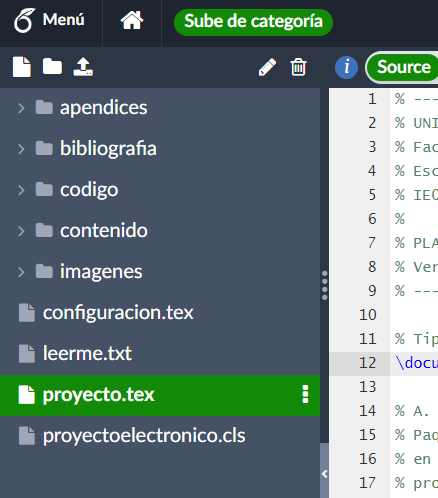
\includegraphics[scale=0.8]{./imagenes/estructura_de_archivos.png}
    \caption{Estructura de archivos de la plantilla.}
    \label{F:estructura_archivos}
\end{figure}



\clearpage
\subsection{Datos generales}

Los datos de la portada y la página de aprobación se ingresan en \texttt{proyecto.tex}. A continuación, se muestra exactamente donde se deben ingresar los datos.

\footnotesize
\begin{lstlisting}[language=TeX, numbers=none]
% Titulo del proyecto
\titulo{Colocar aqui el nombre del proyecto}

% Autor (nombre y carne)
\autoruno{Nombre del primer integrante}
\carneuno{Legajo del primer integrante} % legajo
\emailuno{Email del primer integrante}

\autordos{Nombre del segundo integrante}
\carnedos{Legajo del segundo integrante} % legajo
\emaildos{Email del segundo integrante}

%\autortres{Nombre del tercer integrante}
%\carnetres{Legajo del tercer integrante} % legajo
%\emailtres{Email del tercer integrante}

% Profesor(a) guia
\guia{Nombre del profesor tutor}

% Profesores lectores 
\lectorA{Nombre del primer profesor lector}
\lectorB{Nombre del segundo profesor lector}

% Fecha de entrega del trabajo escrito
\mes{11}	% Numero del mes
\ano{2022}	% Formato AAAA
\end{lstlisting}
\normalsize

Como puede apreciarse existen campos para incluir un tercer integrante al grupo, en caso de ser necesario, descomentar los campos y rellenarlos. Para poder visualizar al tercer integrante en la carátula, página de aprobación, resumen y abstract, debemos dirigirnos a \texttt{proyectoelectronico.cls} y descomentar algunas líneas; las mismas se muestran a continuación. Se recomienda utilizar el buscador (Ctrl + F) para encontrarlas rápidamente.

Estas líneas son de la carátula, y deben ser descomentadas si esperamos que el tercer integrante aparezca en la misma.

\footnotesize
\begin{lstlisting}[language=TeX, numbers=none]
%	\vskip 0.8em
%	\large\bfseries \@autortres \\
%	\vskip 0.1em
%	\large\bfseries \@emailtres \\
\end{lstlisting}
\normalsize

\clearpage
Estas líneas son de la hoja de aprobación, y deben ser descomentadas si esperamos que el tercer integrante aparezca en la misma.

\footnotesize
\begin{lstlisting}[language=TeX, numbers=none]
%	\large\bfseries \@autortres \\
%	\vskip 0.1em
%	\large\bfseries \@emailtres \\
%	\vskip 0.1em
%	\large\bfseries \@carnetres \\
\end{lstlisting}
\normalsize

Esta última línea se repite dos veces, una para el resumen y otra vez para el abstract. La misma debe ser descomentada en ambas partes si esperamos que el tercer integrante aparezca correctamente en ellas.

\footnotesize
\begin{lstlisting}[language=TeX, numbers=none]
%		\large\bfseries\@autortres
\end{lstlisting}
\normalsize

\subsection{Resumen}

Para escribir el resumen\footnote{Recordar que el resumen es una de las cosas que se termina por último, hay que tener el informe escrito casi en su totalidad para saber que escribir en el resumen. En esta sección simplemente se describe como modificarlo, pero debe realizarse por último.} es necesario ir al archivo \texttt{./contenido/resumen.tex}. El contenido actual del mismo se muestra a continuación.
\footnotesize
\begin{lstlisting}[language=TeX]
% EL RESUMEN
% ----------

\begin{resumen}{Aqui, van, las, palabras, claves, separadas, por, comas}

\lipsum[1-2]

\end{resumen}
\end{lstlisting}
\normalsize

Aquí debe agregarse las palabras claves separadas por coma, y luego escribir el resumen en sí. Para ello es necesario eliminar la línea con el comando \texttt{$\backslash$lipsum[1-2]}, el mismo es simplemente un comando para generar texto aleatorio con el objetivo de rellenar plantillas y ver como quedarían si tuviesen texto, por lo tanto, debe eliminarse antes de escribir el resumen.

\clearpage
\subsection{Abstract}

El abstract es simplemente una traducción del resumen y para escribirlo es necesario ir al archivo \texttt{./contenido/abstract.tex}. El contenido actual del mismo se muestra a continuación.
\footnotesize
\begin{lstlisting}[language=TeX]
% EL RESUMEN EN INGLES
% --------------------

\begin{theabstract} {Here goes the translated title of the project} {Here, goes, the, keywords, separated, by, commas}

\lipsum[1-2]

\end{theabstract}
\end{lstlisting}
\normalsize

Su modificación es similar a la del resumen, con la diferencia de que aquí el entorno \entreComillas{theabstract} recibe dos parámetros, primero el título traducido y luego las palabras claves, por supuesto, también en inglés.

Al igual que el resumen, para escribir el abstract es necesario eliminar la línea con el comando \texttt{$\backslash$lipsum[1-2]} antes.

\subsection{Agradecimientos}

Para agregar los agradecimientos es necesario simplemente modificar el archivo: \\ \texttt{./contenido/agradecimientos.tex}.

\subsection{Nomenclatura}

Para modificar las nomenclaturas utilizadas debe modificarse el archivo: \\ \texttt{./contenido/nomenclatura.tex}.

Para ello se utiliza el comando \texttt{$\backslash$nomenclature\{\}\{\}}, el mismo recibe dos parámetros, el primero de ellos es la abreviatura o palabra, y el segundo su significado. En el archivo actual se encuentran muchos ejemplos, los cuales deben ser quitados si no son utilizados y agregar los que sí aplican al informe.

\subsection{Índices}

En el archivo \texttt{proyecto.tex} se encuentra especificado cómo se imprime la tabla de contenidos

\footnotesize
\begin{lstlisting}[language=TeX, numbers=none]
% 5. TABLAS DE CONTENIDO, FIGURAS Y TABLAS
\tableofcontents
\listoffigures
\listoffotos
\listoftables
\lstlistoflistings
\end{lstlisting}
\normalsize

Como hay muchos índices separados, deberíamos retirar los que no utilizamos. Por ejemplo, si no incluimos el código de ningún programa, deberíamos no incluir el índice de listados, es decir, quitar el comando \texttt{$\backslash$lstlistoflistings}.

\clearpage
\subsection{Modificaciones extras}

La idea de utilizar una plantilla es precisamente poder simplemente escribir el documento sin tener que molestarse con los detalles de formateo del mismo. Sin embargo, si es de interés para el alumno realizar modificaciones, mencionamos que en el archivo \texttt{proyectoelectronico.cls} se encuentra formateado la portada:

\footnotesize
\begin{lstlisting}[language=TeX, numbers=none]
% 1. Formato de portada
% ---------------------

\newcommand{\portada}{
...
}
\end{lstlisting}
\normalsize

La hoja de aprobación:

\footnotesize
\begin{lstlisting}[language=TeX, numbers=none]
% 2. Formato de la hoja de aprobacion
% -----------------------------------

\newcommand{\aprobacion}{
...
}
\end{lstlisting}
\normalsize

El resumen:

\footnotesize
\begin{lstlisting}[language=TeX, numbers=none]
% 3. Formato del resumen
% ----------------------

\NewDocumentEnvironment{resumen}{ m }
{
...
}
\end{lstlisting}
\normalsize

El abstract:

\footnotesize
\begin{lstlisting}[language=TeX, numbers=none]
% 4. Formato del abstract
% -----------------------

\NewDocumentEnvironment{theabstract}{ m m }
{
...
}
\end{lstlisting}
\normalsize

La hoja de agradecimientos (llamado reconocimientos en el código):

\footnotesize
\begin{lstlisting}[language=TeX, numbers=none]
% 5. Formato de los reconocimientos
% ---------------------------------

\NewDocumentEnvironment{reconocimiento}{ m }
{
...
}
\end{lstlisting}
\normalsize


\clearpage
\subsection{Agregar un capítulo}

Para agregar un capítulo nuevo creamos un archivo dentro de la carpeta \texttt{./contenido/} haciendo click derecho y seleccionando \entreComillas{Archivo nuevo}, como puede apreciarse en la figura~\ref{F:crear_nuevo_capitulo}.

\begin{figure}[ht]
  \centering
  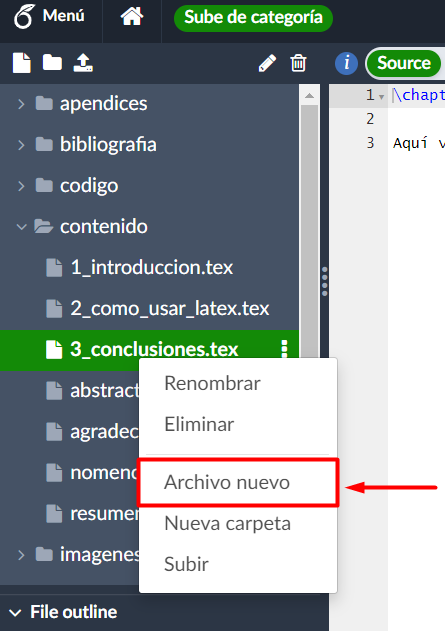
\includegraphics[width=0.45\textwidth]{./imagenes/crear_nuevo_capitulo.png}
  \caption{Creación de nuevo capítulo}
  \label{F:crear_nuevo_capitulo}
\end{figure}

Le asignamos al archivo un nombre apropiado y dentro del mismo utilizamos  \texttt{$\backslash$chapter\{\}}, para definir el capítulo y su nombre.

\footnotesize
\begin{lstlisting}[language=TeX, numbers=none]
\chapter{Nombre del nuevo capitulo}

% Texto de mi nuevo capitulo...
\end{lstlisting}
\normalsize

Dentro de este archivo es donde escribiremos nuestro capítulo. Pero para incluirlo al informe primero debemos dirigirnos al archivo \texttt{proyecto.tex}, y agregarlo con el comando \texttt{$\backslash$input\{\}}, teniendo en cuenta la posición del mismo respecto de los otros capítulos. Como puede observarse en la captura de la figura~\ref{F:nuevo_capitulo}, el mismo se agregó justo seguido de las conclusiones, pero podría ser puesto en otro orden.
\clearpage
\begin{figure}[ht]
  \centering
  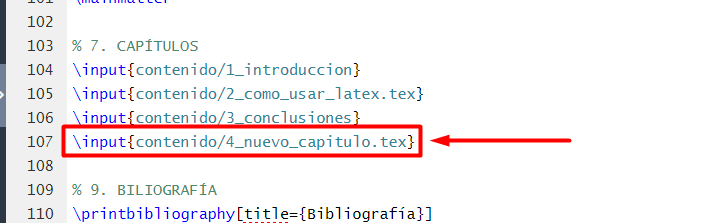
\includegraphics[width=0.85\textwidth]{./imagenes/nuevo_capitulo.png}
  \caption{Creación de nuevo capítulo}
  \label{F:nuevo_capitulo}
\end{figure}

\clearpage
\section{Figuras}

\footnotesize
\begin{lstlisting}
En la figura~\ref{F:diag_bloq_sistema_minimo} puede observarse el diagrama de bloques del sistema minimo.

\begin{figure}[ht]
  \centering
  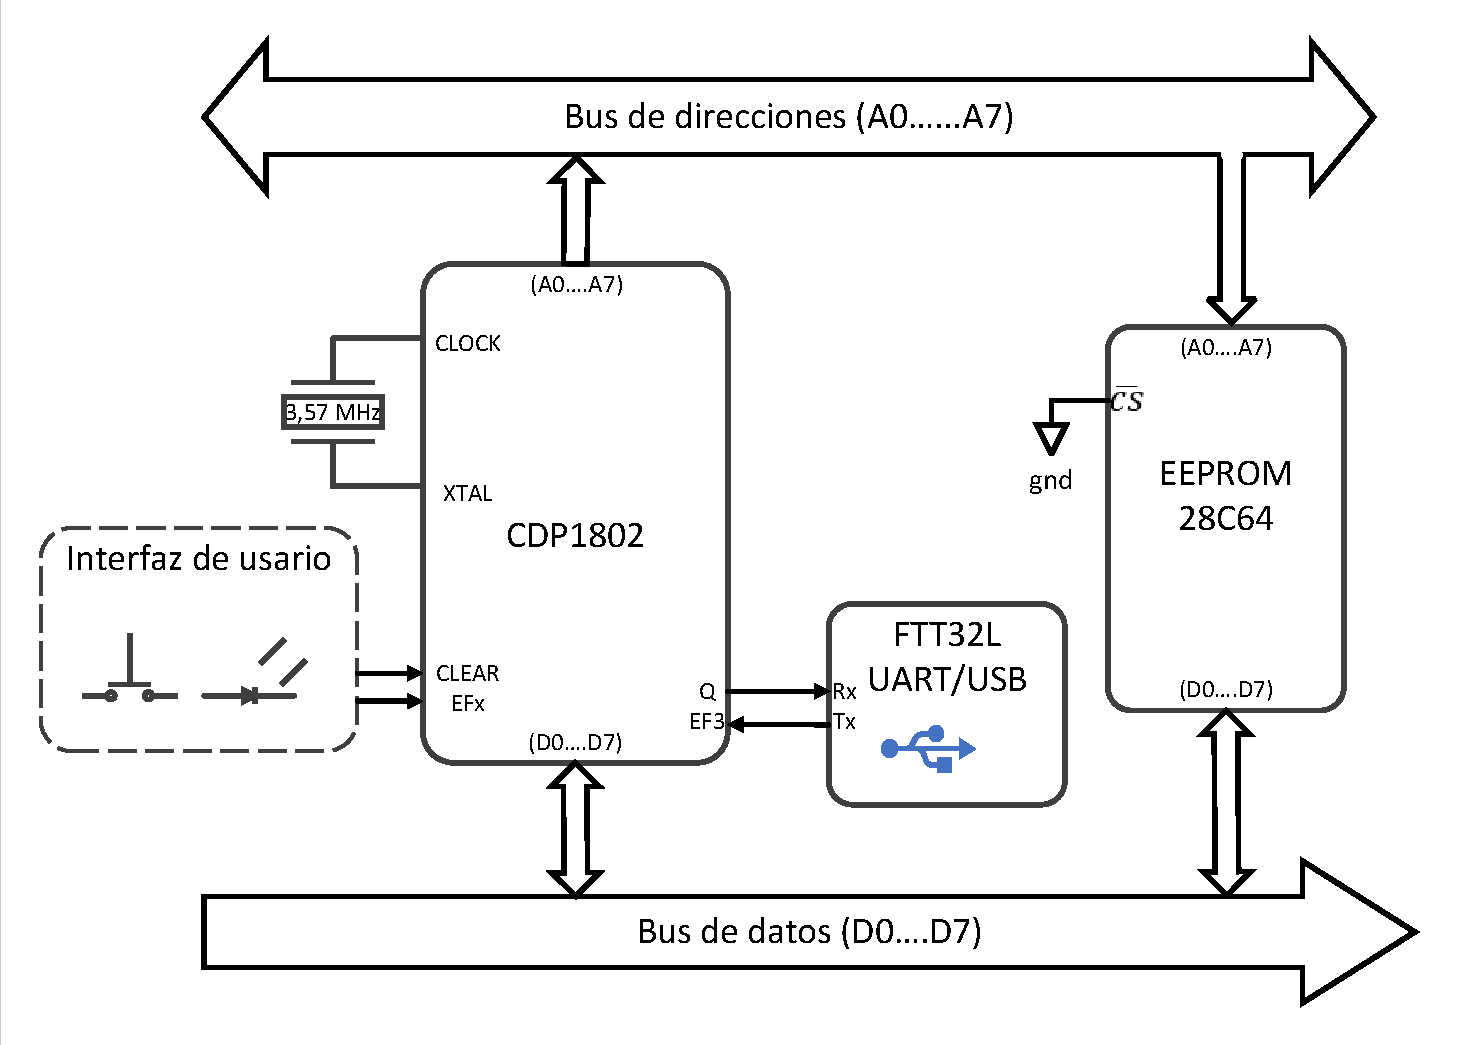
\includegraphics[width=0.9\textwidth]{./imagenes/diag_bloq_sistema_minimo.pdf}
  \caption{Diagrama de bloques del sistema minimo}
  \label{F:diag_bloq_sistema_minimo}
\end{figure}
\end{lstlisting}
\normalsize

En la figura~\ref{F:diag_bloq_sistema_minimo} puede observarse el diagrama de bloques del sistema mínimo.

\begin{figure}[ht]
  \centering
  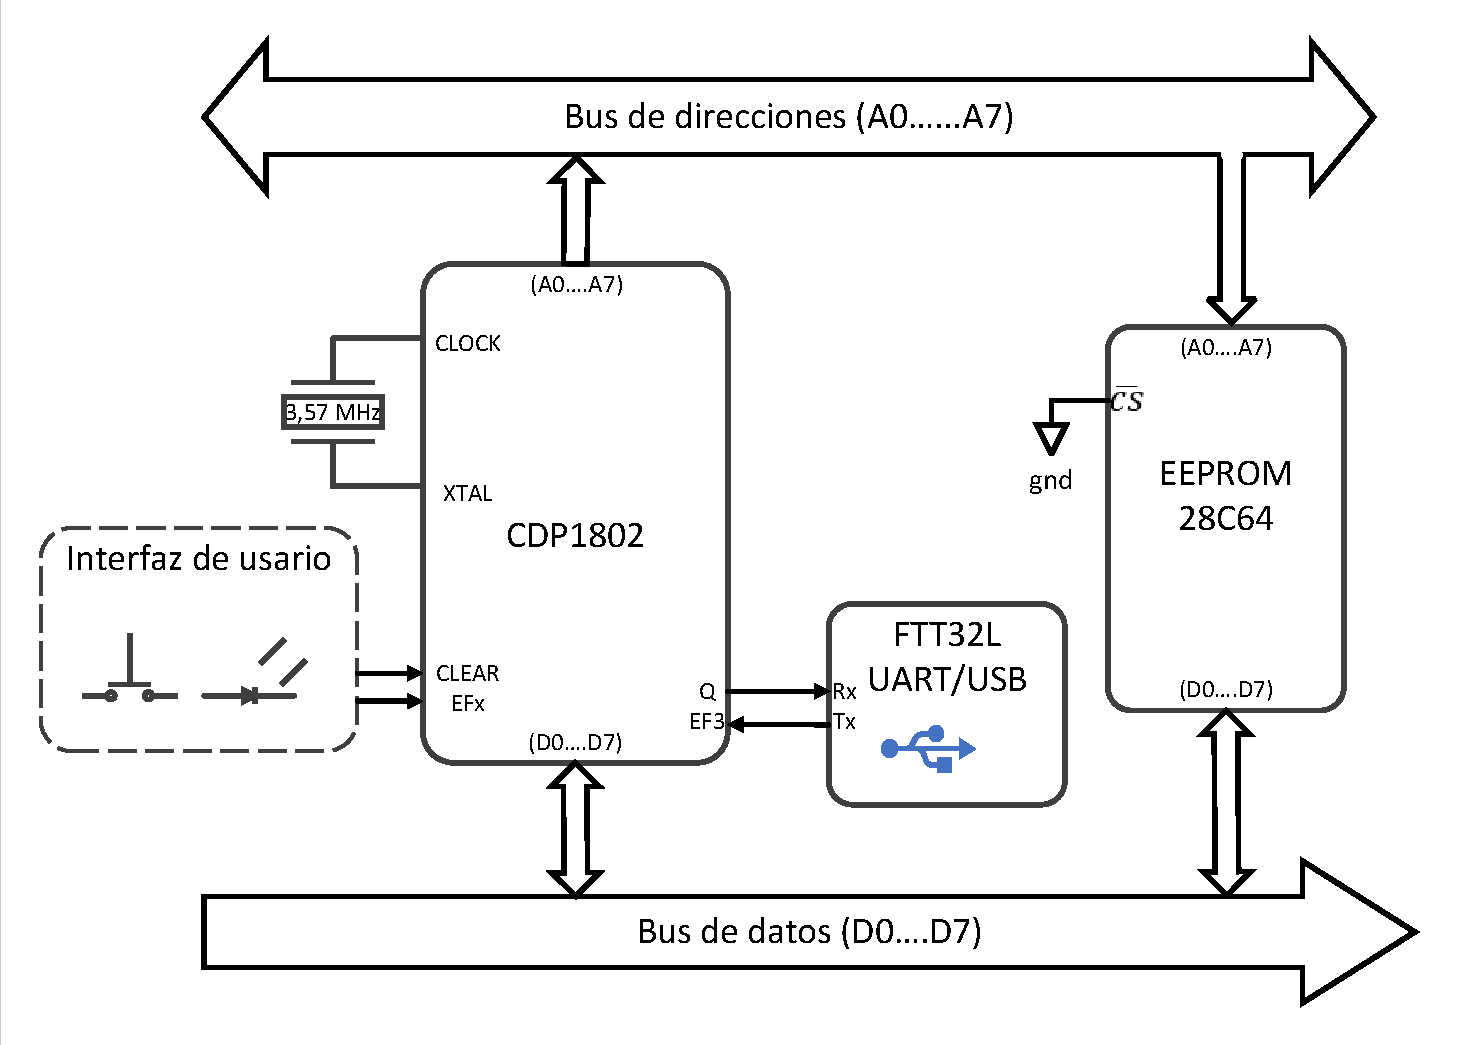
\includegraphics[width=0.9\textwidth]{./imagenes/diag_bloq_sistema_minimo.pdf}
  \caption{Diagrama de bloques del sistema mínimo}
  \label{F:diag_bloq_sistema_minimo}
\end{figure}

\clearpage
\footnotesize
\begin{lstlisting}
\begin{figure}[ht!]
\centering
\subfloat[Transistor (texto que aparece en el indice)][Transistor en encapsulado TO-220]{
	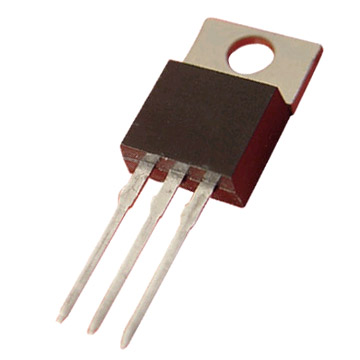
\includegraphics[width=0.2\textwidth]{./imagenes/transistor.jpg}
	\label{F:subfig1}}
\qquad
\subfloat[LED][LED blanco de baja potencia]{
	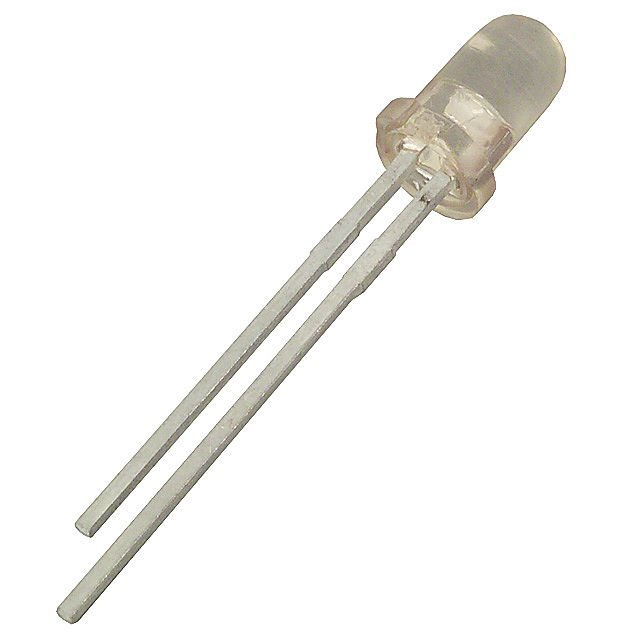
\includegraphics[width=0.2\textwidth]{./imagenes/led.jpg}
	\label{F:subfig2}}
\\
\subfloat[Fotoconductor][Fotoconductor]{
	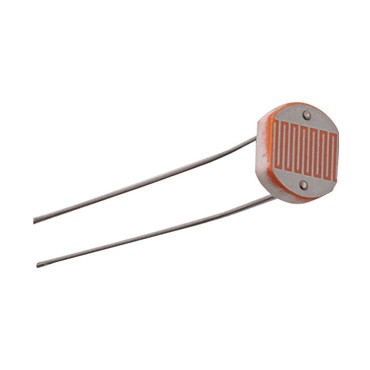
\includegraphics[width=0.2\textwidth]{./imagenes/fotoconductor.jpg}
	\label{F:subfig3}}
\qquad
\subfloat[Circuito integrado][Circuito integrado en encapsulado DIP-8]{
	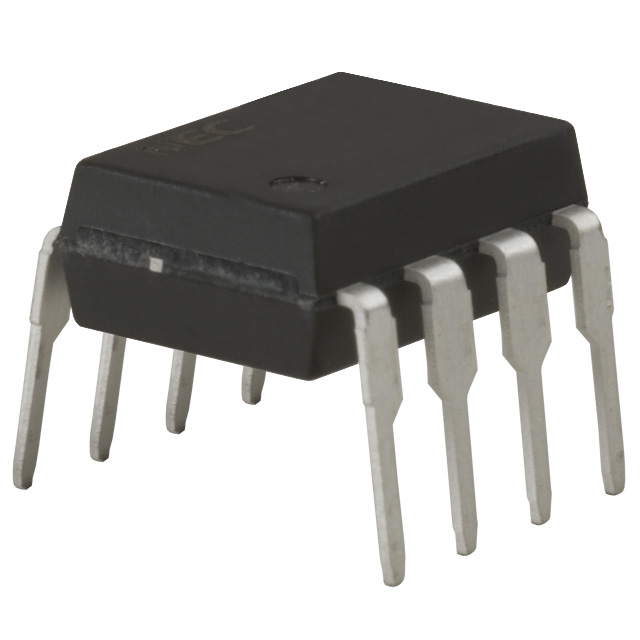
\includegraphics[width=0.2\textwidth]{./imagenes/integrado.jpg}
	\label{F:subfig4}}
\caption{Una figura con varias subfiguras, utilizando el paquete \texttt{subfig}}
\label{F:subfiguras}
\end{figure}
\end{lstlisting}
\normalsize


\begin{figure}[ht!]
\centering
\subfloat[Transistor (texto que aparece en el índice)][Transistor en encapsulado TO-220]{
	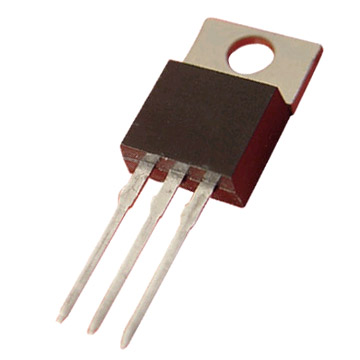
\includegraphics[width=0.2\textwidth]{./imagenes/transistor.jpg}
	\label{F:subfig1}}
\qquad
\subfloat[LED][LED blanco de baja potencia]{
	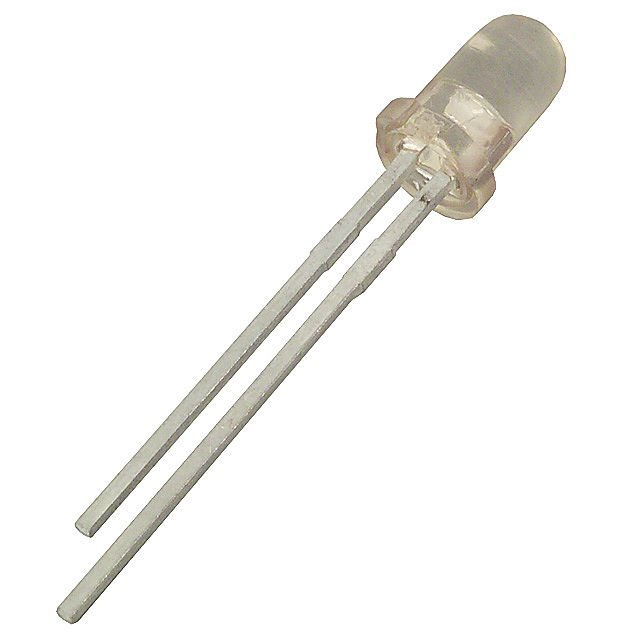
\includegraphics[width=0.2\textwidth]{./imagenes/led.jpg}
	\label{F:subfig2}}
\\
\subfloat[Fotoconductor][Fotoconductor]{
	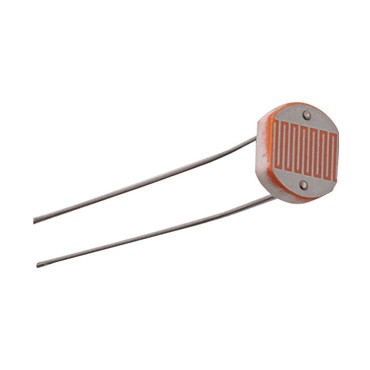
\includegraphics[width=0.2\textwidth]{./imagenes/fotoconductor.jpg}
	\label{F:subfig3}}
\qquad
\subfloat[Circuito integrado][Circuito integrado en encapsulado DIP-8]{
	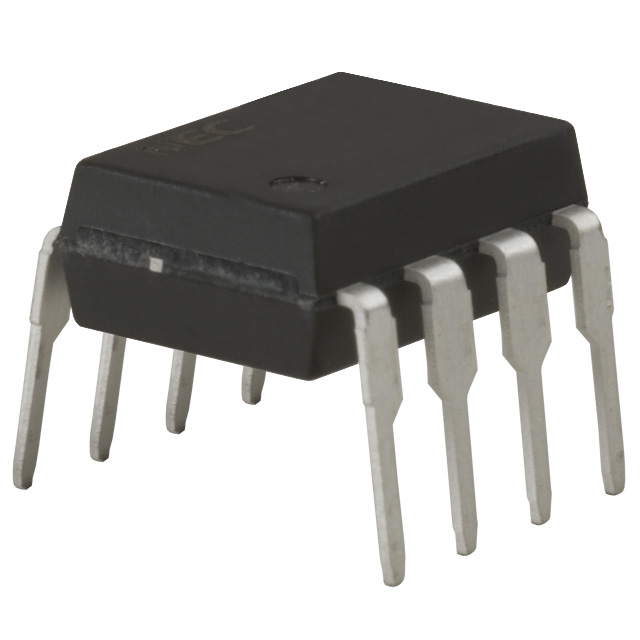
\includegraphics[width=0.2\textwidth]{./imagenes/integrado.jpg}
	\label{F:subfig4}}
\caption{Una figura con varias subfiguras, utilizando el paquete \texttt{subfig}}
\label{F:subfiguras}
\end{figure}

\clearpage
\section{Fotografías}

A pedido de la cátedra se incluyó un entorno distinto al de figuras para presentar fotografías. El mismo se utiliza de igual manera que el entorno de figuras, con la única diferencia de que este entorno se llama \entreComillas{foto}, como se muestra a continuación.

\footnotesize
\begin{lstlisting}
En la fotografia~\ref{F:foto_sistema_med} puede verse el sistema medio construido.

\begin{foto}[ht]
  \centering
  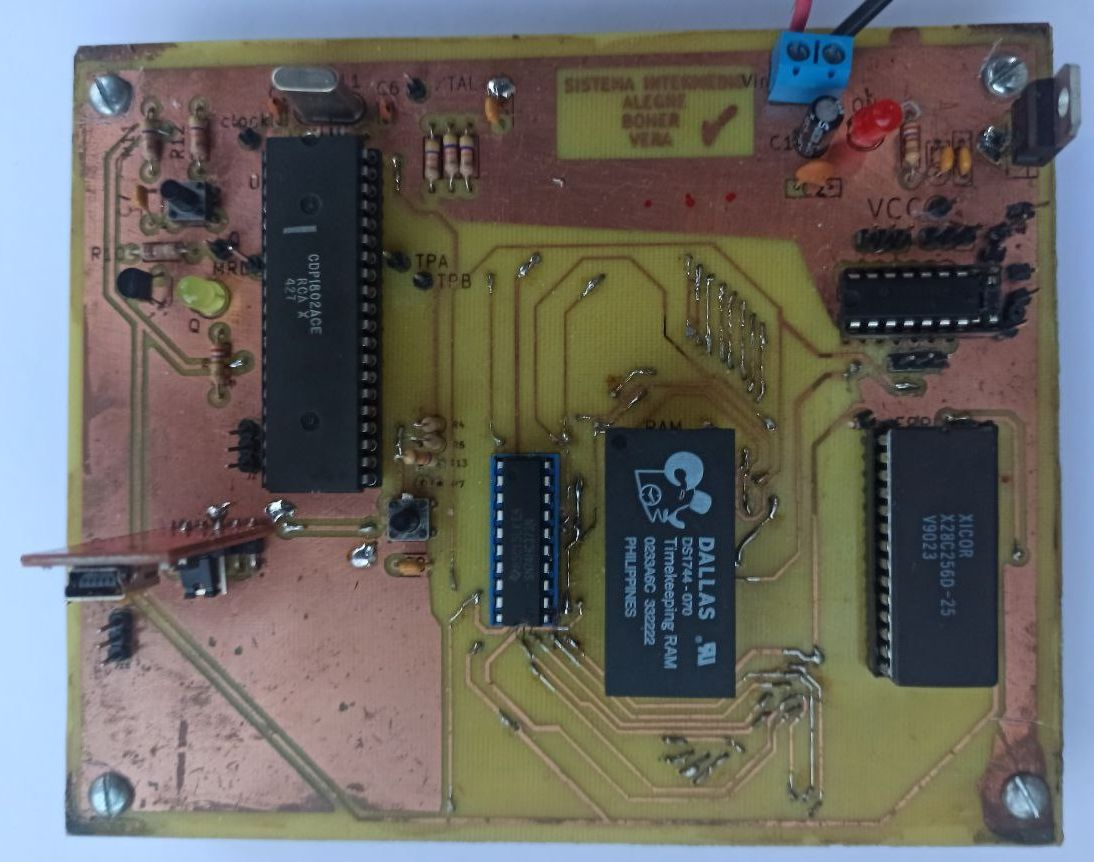
\includegraphics[width=0.9\textwidth]{./imagenes/foto_sistema_med.jpg}
  \caption{Sistema medio construido}
  \label{F:foto_sistema_med}
\end{foto}
\end{lstlisting}
\normalsize

En la fotografía~\ref{F:foto_sistema_med} puede verse el sistema medio construido.

\begin{foto}[ht]
  \centering
  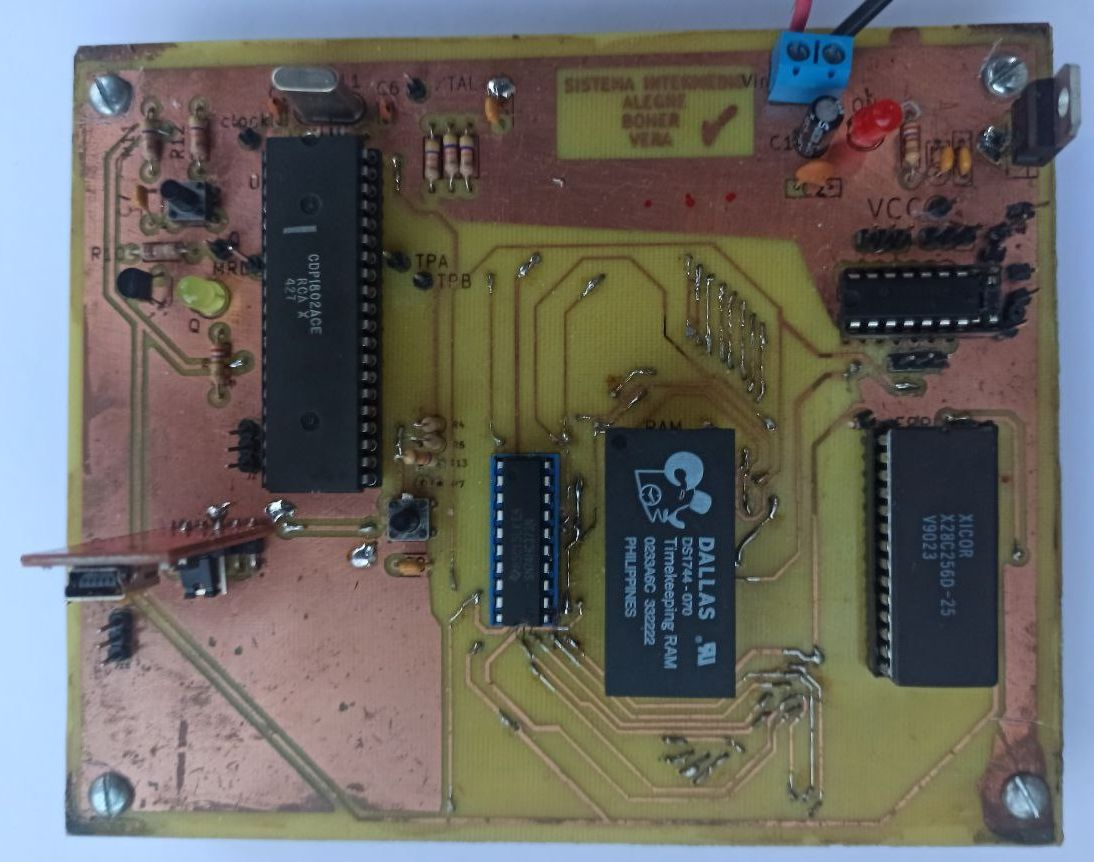
\includegraphics[width=0.9\textwidth]{./imagenes/foto_sistema_med.jpg}
  \caption{Sistema medio construido}
  \label{F:foto_sistema_med}
\end{foto}



\clearpage
\section{Tablas}

A continuación, se muestran algunas tablas como ejemplo. Existen páginas para crear tablas de \LaTeX~de forma rápida y sencilla, como por ejemplo \cite{tablas_latex_online}; el cual se utilizó en varias ocasiones.


\begin{table}[ht!]
\caption{Numeración decimal, binaria y hexadecimal}
\label{T:dec_bin_hex}
\begin{tabular}{|c|c|c|}
\hline
Decimal & Binario & Hexadecimal \\ \hline \hline
0       & 0000    & 0           \\ \hline
1       & 0001    & 1           \\ \hline
2       & 0010    & 2           \\ \hline
3       & 0011    & 3           \\ \hline
4       & 0100    & 4           \\ \hline
5       & 0101    & 5           \\ \hline
6       & 0110    & 6           \\ \hline
7       & 0111    & 7           \\ \hline
8       & 1000    & 8           \\ \hline
9       & 1001    & 9           \\ \hline
10      & 1010    & A           \\ \hline
11      & 1011    & B           \\ \hline
12      & 1100    & C           \\ \hline
13      & 1101    & D           \\ \hline
14      & 1110    & E           \\ \hline
15      & 1111    & F           \\ \hline
\end{tabular}
\end{table}


% Please add the following required packages to your document preamble:
% \usepackage{multirow}
\begin{table}[ht!]
\caption{Códigos de estado}
\label{T:state_codes}
\begin{tabular}{|l|ll|}
\hline
\multicolumn{1}{|c|}{\multirow{2}{*}{State Type}} & \multicolumn{2}{l|}{State Code} \\ \cline{2-3} 
\multicolumn{1}{|c|}{}                            & \multicolumn{1}{l|}{SC1}  & SC0 \\ \hline
S0 (Fetch)                                        & \multicolumn{1}{l|}{L}    & L   \\ \hline
S1 (Execute)                                      & \multicolumn{1}{l|}{L}    & H   \\ \hline
S2 (DMA)                                          & \multicolumn{1}{l|}{H}    & L   \\ \hline
S3 (Interrupt)                                    & \multicolumn{1}{l|}{H}    & H   \\ \hline
\end{tabular}
\end{table}


\clearpage

La tabla~\ref{T:bom_sis_final} es un ejemplo de cómo realizar una tabla que es tan grande que se extiende en varias páginas. La misma tiene un encabezado que se repite en cada página, de manera que no es necesario ir al comienzo de la tabla para ver a qué corresponde cada columna, dado que el encabezado está presente al inicio de cada página.

\footnotesize
\begin{longtable}{|P{0.08\textwidth}|P{0.11\textwidth}|P{0.30\textwidth}|P{0.14\textwidth}|P{0.15\textwidth}|}
\caption{Lista de componentes del sistema final} % needs to go inside longtable environment
\label{T:bom_sis_final}
\\
\hline
Cantidad & Etiqueta \newline
           Identificador            & Descripción                               & Fabricante            & Número de parte       \\ \hline \hline \endfirsthead
\hline
Cantidad & Etiqueta \newline
           Identificador            & Descripción                               & Fabricante            & Número de parte       \\ \hline \hline \endhead
1       & U1                        & Microprocesador                           & RCA                   & CDP1802ACE            \\ \hline
1       & U2                        & Latch de 8 bits                           & Philips               & 74HC573N              \\ \hline
1       & U3                        & Memoria EEPROM 32k x 8                    & XICOR                 & X28C256D-25           \\ \hline
1       & U4                        & Memoria EEPROM Serial I2C 128k x 8        & Microchip             & 24LC1025              \\ \hline
1       & U5                        & Time keeping RAM 32K x8                   & Dallas                & DS1744-070            \\ \hline
1       & U6                        & Memoria RAM 32k x 8                       & HYUNDAI               & HY62256ALP-10         \\ \hline
1       & U7                        & Memoria FRAM Serial I2C 8k x 8            & Fujitsu Semiconductors & MB85RC64A            \\ \hline
1       & U8                        & Conversor analógico-digital con interfaz I2C & Maxim Integrated   & MAX127                \\ \hline
1       & U9                        & Regulador de tensión 12~\si{\volt}        & Motorola              & 7812CT                \\ \hline
1       & U10                       & Regulador de tensión 5~\si{\volt}         & ST Microelectronics   & L7805CV               \\ \hline
1       & U11                       & High Precision Operational Amplifier      & Burr Brown            & OPA4277PA             \\ \hline
1       & U12                       & Regulador de tensión -12~\si{\volt}       & ST Microelectronics   & L7912CV               \\ \hline
5       & U13, U14, U15, U16, U28   & Cuadruple compuerta NAND de dos entradas  & Texas Instrument      & SN74HC00N             \\ \hline
1       & U17                       & Cuadruple compuerta NAND de dos entradas con Schmitt-Trigger & Texas Instrument & SN74HC132N \\ \hline
2       & U18,U30                   & Cuadruple compuerta NOR de dos entradas   & Texas Instrument      & SN74HC02N             \\ \hline
1       & U19                       & Decodificador Multiplexador 3 a 8 líneas  & Texas Instrument      & SN74HC138N            \\ \hline
1       & U20                       & CMOS Programmable Peripheral Interface    & Intersil              & CP82C55A-5Z           \\ \hline
1       & U21                       & Regulador programable shunt               & Fairchild             & LM336Z25              \\ \hline
1       & U24                       & Doble flip-flop tipo D con Set y Reset    & Texas Instrument      & SN74HC74N             \\ \hline
1       & U25                       & Contador binario de 4 bits                & Fairchild Semiconductor & MM74HC161N          \\ \hline
1       & U29                       & Doble flip-flop JK con Set y Reset        & National Semiconductors & MM74HC73N           \\ \hline
1       & U31                       & Registro de desplazamiento de 8 bits      & Texas Instrument      & SN74HC595N            \\ \hline
1       & U32                       & Registro de desplazamiento de 8 estados   & Motorola              & MC14014BCP            \\ \hline
1       & X2                        & XO-22BE-4MHz                              &   \listaVacio                    & \listaVacio                      \\ \hline
1       & XTAL1                     & Cristal \num{4}~\si{\mega\hertz}          & CQ Electronics        & \listaVacio                      \\ \hline
1       & SW1                       & Llave DPDT 6 pines                        & \listaVacio                      & \listaVacio                      \\ \hline
3       & SW2, SW3, SW4             & Pulsador 6mm~x~4,3mm                      &  \listaVacio                     &  \listaVacio                     \\ \hline
5       & T2, T3, T4, T5, T6        & Transistor BJT NPN                        & Motorola              & P2N2222A               \\ \hline
1       & RV1                       & Preset 10~\si{\kilo\ohm}                  &  \listaVacio                     &  \listaVacio                     \\ \hline
1       & D1                        & Puente rectificador de onda completa B380R &            \listaVacio           &  \listaVacio                     \\ \hline
6       & D2, D3, D4, D5, D6, D7    & LED 5~mm                                  &\listaVacio                       &   \listaVacio                    \\ \hline
2       & D8, D9                    & 1N914                                     &\listaVacio                       &  \listaVacio                     \\ \hline
1       & F1                        & Fusible 10~mm 1~\si{\ampere}              &\listaVacio                       &  \listaVacio                     \\ \hline
8       & R1, R2, R3, R5, R21, R22, R23, R27
                                    & Resistor 47~\si{\kilo\ohm} 1/8~\si{\watt} & \listaVacio                      &   \listaVacio                    \\ \hline
1       & R4                        & Resistor 10~\si{\mega\ohm} 1/8~\si{\watt} &  \listaVacio                     &   \listaVacio                    \\ \hline
1       & R6                        & Resistor 330~\si{\ohm} 1/4~\si{\watt}     &  \listaVacio                     &   \listaVacio                    \\ \hline
2       & R7, R8                    & Resistor 1~\si{\kilo\ohm} 1/8~\si{\watt}  &  \listaVacio                     &    \listaVacio                   \\ \hline
3       & R9, R10, R11              & Resistor 220~\si{\ohm} 1/4~\si{\watt}     &    \listaVacio                   &    \listaVacio                   \\ \hline
16      & R12, R13, R14, R15, R16, R17, R18, R38, R39, R40, R41, R46, R47, R56, R57, R60
                                    & Resistor 10~\si{\kilo\ohm} 1/8~\si{\watt} & \listaVacio                      &   \listaVacio                    \\ \hline
5       & R19, R20, R24, R25, R26   & Resistor 100~\si{\kilo\ohm} 1/8~\si{\watt}&  \listaVacio                     &   \listaVacio                    \\ \hline
4       & R28, R30, R36, R52        & Resistor 100~\si{\ohm} 1/4~\si{\watt}     &  \listaVacio                     &   \listaVacio                    \\ \hline
4       & R29, R31, R37, R53        & Resistor 150~\si{\ohm} 1/4~\si{\watt}     &  \listaVacio                     &   \listaVacio                    \\ \hline
8       & R32, R33, R34, R35, R42, R43, R54, R55
                                    & Resistor 390~\si{\kilo\ohm} 1/8~\si{\watt}&  \listaVacio                     & \listaVacio                      \\ \hline
8       & R44, R45, R48, R49, R50, R51, R58, R59
                                    & Resistor 1~\si{\mega\ohm} 1/8~\si{\watt}  &  \listaVacio                     & \listaVacio                      \\ \hline
2       & C2, C3                    & Capacitor cerámico \num{30}~\si{\pico\farad} 50~\si{\volt}
                                                                                &   \listaVacio                    & \listaVacio                      \\ \hline
14       & C5, C7, C8, C29, C30, C31, C14, C15, C18, C32, C33, C39, C40, C43
                                    & Capacitor cerámico \num{0.10}~\si{\micro\farad} 50~\si{\volt}
                                                                                &    \listaVacio                   &   \listaVacio                    \\ \hline
1       & C11, C17                  & Capacitor electrolítico 4700~\si{\micro\farad} 25~\si{\volt}
                                                                                &     \listaVacio                  &   \listaVacio                    \\ \hline
2       & C12, C16                  & Capacitor cerámico \num{0.33}~\si{\micro\farad} 50~\si{\volt}
                                                                                &   \listaVacio                    &  \listaVacio                     \\ \hline
1       & C13                       & Capacitor electrolítico 10~\si{\micro\farad} 25~\si{\volt}
                                                                                &   \listaVacio                    &  \listaVacio                     \\ \hline
1       & C19                       & Capacitor electrolítico \num{0.01}~\si{\micro\farad} 25~\si{\volt}
                                                                                &     \listaVacio                  &  \listaVacio                     \\ \hline
1       & C20                       & Capacitor electrolítico \num{4.7}~\si{\micro\farad} 25~\si{\volt}
                                                                                &   \listaVacio                    &  \listaVacio                     \\ \hline
6       & J1, J2, J33, J48, J49, J50& 1x3 Pines Conectores Macho \num{2.54}~mm  &   \listaVacio                    &  \listaVacio                     \\ \hline
38      & J3, J4, J5, J6, J7, J8, J9, J10, J11, J12, J13, J14, J15, J16, J17, J18, J19, J20, J21, J22, J23, J24, J25, J26, J27, J28, J29, J30, J31, J36, J40, J41, J42, J45, J46, J51, J52, J53
                                    & Pin conector macho (1 \textit{Male Header Pin}) & \listaVacio                      &   \listaVacio                    \\ \hline
3       & J32, J35, J38             & 1x6 Pines Conectores Macho \num{2.54}~mm  & \listaVacio                      & \listaVacio                      \\ \hline
3       & J34, J37, J39             & 1x5 Pines Conectores Macho \num{2.54}~mm  & \listaVacio                      &   \listaVacio                    \\ \hline
2       & J43, J44                  & Bornera 3 pines \num{5.08}~mm             &  \listaVacio                     &  \listaVacio                     \\ \hline
2       & J47, J54                  & 1x12 Pines Conectores Macho \num{2.54}~mm &   \listaVacio                    &  \listaVacio                     \\ \hline
1       & J55                       & 1x2 Pines Conectores Macho \num{2.54}~mm  &   \listaVacio                    &   \listaVacio                    \\ \hline
1       & No aplica                 & Módulo conversor USB-Serial               & Future Technology Devices International & FT232RL \\ \hline
1       & No aplica                 & Módulo adaptador tarjeta micro SD         & \listaVacio  & \listaVacio \\ \hline
\end{longtable}
\normalsize

\clearpage
\section{Números y Unidades}

A continuación, se muestra como escribir unidades de forma correcta.


\begin{lstlisting}[language=TeX, numbers=none]
Las unidades se escriben utilizando el paquete siunitx. Puede ser asi: \SI{2.2}{\kilo\ohm}, o tambien ser asi: \num{2.2} \si{\kilo\ohm}.
\end{lstlisting}
\normalsize

Si compilamos esto, obtenemos:

Las unidades se escriben utilizando el paquete siunitx. Puede ser así: \SI{2.2}{\kilo\ohm}, o también ser así: \num{2.2} \si{\kilo\ohm}.

\vspace{1cm}

Pero es importante utilizar correctamente el espacio de no separación \textasciitilde~(que es el carácter 126 del código ASCII) para separar el número de la unidad, si se escriben por separado. De esta manera se evita que en los saltos de línea se separe el número de la unidad. Reescribamos lo anterior pero esta vez con un espacio de no separación.


\begin{lstlisting}[language=TeX, numbers=none]
Las unidades se escriben utilizando el paquete siunitx. Puede ser asi: \SI{2.2}{\kilo\ohm}, o tambien ser asi: \num{2.2}~\si{\kilo\ohm}.
\end{lstlisting}
\normalsize

Si compilamos esto, obtenemos:

Las unidades se escriben utilizando el paquete siunitx. Puede ser asi: \SI{2.2}{\kilo\ohm}, o tambien ser asi: \num{2.2}~\si{\kilo\ohm}.

\vspace{1cm}

Como vemos, ahora no se separó el número de la unidad.

\clearpage
\section{Ecuaciones}

\footnotesize
\begin{lstlisting}
En la ecuacion~\eqref{eq:ecuacion_1} se encuentra la formula de Euler.

\begin{equation}
\label{eq:ecuacion_1}
 e^{jx} = \cos{x} + j \sin{x}
\end{equation}
\end{lstlisting}
\normalsize

En la ecuación~\eqref{eq:ecuacion_1} se encuentra la fórmula de Euler.

\begin{equation}
\label{eq:ecuacion_1}
 e^{jx} = \cos{x} + j \sin{x}
\end{equation}

\footnotesize
\begin{lstlisting}
\begin{equation}
u(x) = 
  \begin{cases} 
   \exp{x} & \text{si } x \geq 0 \\
   1       & \text{si } x < 0
  \end{cases}
\end{equation}
\end{lstlisting}
\normalsize

\begin{equation}
u(x) = 
  \begin{cases} 
   \exp{x} & \text{si } x \geq 0 \\
   1       & \text{si } x < 0
  \end{cases}
\end{equation}

\footnotesize
\begin{lstlisting}
\begin{subequations}
    \begin{equation}
    r_1^2 = (h_T-h_R)^2+d^2
    \label{eq: r1_tierra_plana}
    \end{equation}
    \begin{equation}
    r_2^2 = (h_T+h_R)^2+d^2
    \label{eq: r2_tierra_plana}
    \end{equation}
\end{subequations}
\end{lstlisting}
\normalsize

\begin{subequations}
    \begin{equation}
    r_1^2 = (h_T-h_R)^2+d^2
    \label{eq: r1_tierra_plana}
    \end{equation}
    \begin{equation}
    r_2^2 = (h_T+h_R)^2+d^2
    \label{eq: r2_tierra_plana}
    \end{equation}
\end{subequations}


\clearpage
\section{Código fuente}

Código fuente puede ser ingresado de la siguiente manera.

\footnotesize
\begin{lstlisting}
En el listado~\ref{L:codigo_ejemplo} puede verse en codigo de ejemplo en Octave.

\footnotesize
\lstinputlisting[language=Octave, caption = {Codigo de ejemplo en Octave}, label = {L:codigo_ejemplo}]{codigo/codigo_ejemplo.m}
\normalsize
\end{lstlisting}
\normalsize

En el listado~\ref{L:codigo_ejemplo} puede verse en código de ejemplo en Octave.

\footnotesize
\lstinputlisting[language=Octave, caption = {Código de ejemplo en Octave}, label = {L:codigo_ejemplo}]{codigo/codigo_ejemplo.m}
\normalsize

También es posible definir un resaltado de sintaxis personalizado. Fue necesario definir uno para el lenguaje ensamblador del microprocesador CDP1802; así que presentamos el mismo como ejemplo. El archivo que define la sintaxis se encuentra en \texttt{./codigo/definiciondeASM.tex}, y para incluirlo debemos dirigirnos a \texttt{proyectoelectronico.cls} y añadir el mismo con el comando \texttt{$ \backslash$input\{\}}, como se muestra a continuación (debe ser luego de haber incluido el paquete \entreComillas{listings}).

\footnotesize
\begin{lstlisting}
\usepackage{listings}
%% este código define el estilo para el lenguaje assembler del CDP1802

\lstdefinelanguage{CDP1802}{
    morekeywords=[1]{LDN, LDA, LDX, LDXA, LDI, STR, STXD,
        INC, DEC, IRX, GLO, PLO, GHI, PHI,
        OR, ORI, XOR, XRI, AND, ANI, SHR, SHCR, RSHR, SHL, SHLC, RSHL,
        ADD, ADI, ADC, ADCI, SD, SDI, SDB, SDBI, SM, SMI, SMB, SMBI,
        BR, NBR, BZ, BNZ, BDF, BPZ, BGE, BNF, BM, BL, BQ, BNQ, B1, BN1, B2, BN2, B3, BN3, B4, BN4,
        LBR, NLBR, LBZ, LBNZ, LBDF, LBNF, LBQ, LBNQ,
        SKP, LSKP, LSZ, LSNZ, LSDF, LSNF, LSQ, LSNQ, LSIE,
        IDL, NOP, SEP, SEX, SEQ, REQ, SAV, MARK, RET, DIS,
        OUT1, OUT2, OUT3, OUT4, OUT5, OUT6, OUT7, INP1, INP2, INP3, INP4, INP5, INP6, INP7, OUT, INP},%
    morekeywords=[2]{r0, r1, r2, r3, r4, r5, r6, r7, r8, r9, r10, r11, r12, r13, r14, r15, ra, rb, rc, rd, re, rf},%
    morekeywords=[3]{org,def,equ,db,dw,include,dseg,cseg,eseg},%
    sensitive=false, % keywords are not case-sensitive
    morecomment=[l]{;}, % l is for line comment
} %

\definecolor{MyDarkGreen}{rgb}{0.0,0.4,0.0} % This is the color used for comments

\lstset{language=CDP1802,
        frame=single, % Single frame around code
        basicstyle=\small\ttfamily, % Use small true type font
        keywordstyle=\color{Blue}\textbf, % Instructions in blue, bold
        keywordstyle=[2]\color{Orange}, % Registers in orange
        keywordstyle=[3]\color{Purple}, % Directives in purple
        commentstyle=\usefont{T1}{pcr}{m}{sl}\color{MyDarkGreen}\small,
        tabsize=4, % 4 spaces per tab
        numbers=left, % Line numbers on left
        firstnumber=1, % Line numbers start with line 1
        numberstyle=\tiny\color{Blue}, % Line numbers are blue and small
        stepnumber=5 % Line numbers go in steps of 5
        } % en este archivo esta la definicion para el estilo de texto en asembler del CDP1802
\end{lstlisting}
\normalsize

Ahora ya podemos utilizar nuestra sintaxis personalizada como se muestra a continuación.

\clearpage

\footnotesize
\begin{lstlisting}
\footnotesize
\lstinputlisting[language=CDP1802, caption = {Rutina de retardo de 1 bit-time}, label = {L:retardo}]{codigo/delay_routine.asm}
\normalsize
\end{lstlisting}
\normalsize

\footnotesize
\lstinputlisting[language=CDP1802, caption = {Rutina de retardo de 1 bit-time}, label = {L:retardo}]{codigo/delay_routine.asm}
\normalsize

\clearpage
\section{Bibliografía}

Los elementos de la bibliografía se encuentran en el archivo \texttt{./bibliografia/bibliografia.bib}, puede abrir el mismo para ver las referencias utilizadas en esta plantilla.


\footnotesize
\begin{lstlisting}
Para citar una referencia se utiliza el comando \cite{plantilla_universidad_de_costa_rica}, y se ingresa la etiqueta de la referencia que deseamos incluir.
\end{lstlisting}
\normalsize

Para citar una referencia se utiliza el comando \cite{plantilla_universidad_de_costa_rica}, y se ingresa la etiqueta de la referencia que deseamos incluir.

Para administrar la bibliografía se recomienda utilizar un programa específico llamado JabRef\cite{jabref}.

